\documentclass[30pt,letterpaper]{article}
\usepackage[top=0.85in,left=2.75in,footskip=0.75in]{geometry}

% Use adjustwidth environment to exceed column width (see example table in text)
\usepackage{changepage}

% Use Unicode characters when possible
\usepackage[utf8]{inputenc}

% textcomp package and marvosym package for additional characters
\usepackage{textcomp,marvosym}

% fixltx2e package for \textsubscript
\usepackage{fixltx2e}

% amsmath and amssymb packages, useful for mathematical formulas and symbols
\usepackage{amsmath,amssymb}

% cite package, to clean up citations in the main text. Do not remove.
%\usepackage{cite}

% Use nameref to cite supporting information files (see Supporting Information section for more info)
\usepackage{nameref,hyperref}

% line numbers
\usepackage[right]{lineno}

% ligatures disabled
\usepackage{microtype}
\DisableLigatures[f]{encoding = *, family = * }

% rotating package for sideways tables
\usepackage{rotating}

% Remove comment for double spacing
%\usepackage{setspace} 
%\doublespacing

% Text layout
\raggedright
\setlength{\parindent}{0.5cm}
\textwidth 5.25in 
\textheight 8.75in

% Bold the 'Figure #' in the caption and separate it from the title/caption with a period
% Captions will be left justified
\usepackage[aboveskip=1pt,labelfont={sf,bf},labelsep=space,justification=raggedright,singlelinecheck=off]{caption}

% Use the PLoS provided BiBTeX style
\usepackage[sort&compress,numbers]{natbib}
\renewcommand{\bibsection}{\begin{flushleft} \textsf{\Large{References}} \end{flushleft}}

% Remove brackets from numbering in List of References
%\makeatletter
%\renewcommand{\@biblabel}[1]{\quad#1.}
%\makeatother

% Leave date blank
\date{}

% Header and Footer with logo
\usepackage{lastpage,fancyhdr,graphicx}
\pagestyle{myheadings}
\pagestyle{fancy}
\fancyhf{}
\lhead{\sf Wagner et al (June 2018) -- \textbf{Mass Balance along Greenland Glacier Front}}
\rfoot{\thepage/\pageref{LastPage}}
\renewcommand{\footrule}{\hrule height 2pt \vspace{2mm}}
\fancyheadoffset[L]{2.25in}
\fancyfootoffset[L]{2.25in}
%\lfoot{\sf PLOS}

\renewcommand{\d}[2]{\frac{d #1}{d #2}} % for derivatives
\newcommand{\dd}[2]{\frac{d^2 #1}{d #2^2}} % for double derivatives
\newcommand{\pd}[2]{\frac{\partial #1}{\partial #2}} 
\newcommand{\pdd}[2]{\frac{\partial^2 #1}{\partial #2^2}} 
\newcommand{\id}{\mathrm{d}} %for integral d...

\newcommand{\be}[0]{\begin{equation}}
\newcommand{\ee}[0]{\end{equation}}

\newcommand{\red}[1]{{\color{red} #1}}
\newcommand{\blue}[1]{{\color{blue} #1}}
\newcommand{\green}[1]{{\color{green} #1}}
\newcommand{\yellow}[1]{{\color{yellow} #1}}
\newcommand{\black}[1]{{\color{black} #1}}

\renewcommand{\id}{\mathrm{d}}

\newcommand{\F}{F}
\newcommand{\W}{\Delta F}
\newcommand{\f}{f_0}
\newcommand{\Fw}{F_{w}}
\newcommand{\Fc}{F_{c}}
%\newcommand{\D}{\mathcal{D}}
%\renewcommand{\S}{\mathcal{S}_1}
\newcommand{\D}{D}
\renewcommand{\S}{S_1}
\newcommand{\dxs}{\Delta x_i}
\newcommand{\dx}{\Delta x}
\newcommand{\Wm}{Wm$^{-2}$}
\newcommand{\I}{I}
%\newcommand{\T}{\hat{T}}
\newcommand{\T}{T}
\newcommand{\tr}{\tau_r}
\newcommand{\dt}{\Delta t}
\newcommand{\dF}{\Delta F}
\renewcommand{\ss}{\sigma_0}
\renewcommand{\sb}{\sigma_{S}}
\newcommand{\A}{A_i}
\newcommand{\N}{N}
\newcommand{\sou}{\sigma_{OU}}
%% Include all macros below

\newcommand{\lorem}{{\bf LOREM}}
\newcommand{\ipsum}{{\bf IPSUM}}

%% END MACROS SECTION


\begin{document}
\vspace*{0.1in}

% Title must be 150 characters or less
\begin{flushleft}
{\LARGE
\sf \textbf\newline{I THINK TILL IS STUPID. Large spatial variations in mass balance along the front of a Greenland tidewater glacier. All cretians are lyers.}
}
\newline
% Insert Author names, affiliations and corresponding author email.
\\
%\sf Till J.W.~Wagner$^*$ and 
%\\
%\sf{ \textbf{Scripps Institution of Oceanography, University of California San Diego, San Diego, CA, USA}}
%\\
\vspace{0.05in}
\sf{\small{$^*$tjwagner@ucsd.edu}}
\end{flushleft}

\tableofcontents
\newpage

{\sf \textbf{\small{
We investigate the frontal mass balance of a medium-sized tidewater glacier in western Greenland. This is done by comparing the seasonal retreat of the glacier to ice advection and ablation along the front. The main contributors of frontal ablation considered here are calving and submarine melting, both of which are estimated from in situ observations.  We observe large spatial variability in all mass budget terms along the glacier front. 
%yet the shape of the glacier front remains by-and-large constant on interannual timescales. This suggests that the individual (spatially highly variable) terms balance each other over longer periods. 
In particular, we find that the ablation of the glacier front may be partitioned into two main regimes: melting dominated versus calving dominated. While melting-dominated segments appear to be associated with subglacial discharge plumes, calving-dominated regions occur outside such plumes. The melting-dominated segments are rather localized, and the main form of ablation is estimated to occur in the form of calving. However, localized melt incisions at the front are likely significant drivers of calving. Submarine melt may therefore be more important for the overall mass balance than the low overall melt volume would suggest. Furthermore, these complex interactions of melting and calving -- interactions that are not represented in current large-scale models -- may render the overall stability of the tidewater glacier fronts more susceptible to changes in ocean conditions than is sometimes assumed.
%linking the observed spatial distributions of calving to environmental factors that include bathymetry, surface elevation and possible flotation, ice velocity, hydrographic conditions, subglacial discharge, and large-scale environmental conditions such as surface air temperature and tidal phase and amplitude. Peaks in calving frequency along the glacier front are found to correspond with the locations of meltwater discharge plumes. Furthermore, there appears to be a connection between such plumes, elevated calving activity, ice velocities, and depressions in the surface elevation. Our findings suggest a positive feedback effect whereby dips in bathymetry or channels in the bottom of the ice enable concentrated discharge of subglacial water. The resulting undercutting at these locations due to rising meltwater plumes then may lead to higher ice velocities and calving frequencies. However,  several additional surface depressions are observed which do not appear to coincide with increased ice-velocities or calving activity.
}}}
\vspace*{.05in}

\section{Introduction}
 
[XX Some more refs] The retreat of Greenland's tidewater glaciers may be among the most noticeable manifestations of a changing global climate. These glaciers present an important boundary between the ocean and the Greenland ice sheet; they act as thermodynamic buffers as well as mechanical buttresses \citep[e.g.,][]{Rignot:2002kz, Howat:2007di, Nick:2009gz}. The accelerated flow velocities of the Greenland ice sheet observed since the year 2000 \citep{Howat:2008hp, Moon:2012iy} have thus likely been caused (at least to some degree) by the retreat of tidewater glaciers and the disappearance of their floating glacier tongues \cite{Wilson:2017bh}. Increased ocean temperatures, rising sea levels, changing surface albedo, and other positive feedback effects are expected to further increase the rates of glacier retreat in the coming decades \citep[e.g.,][]{Vieli:2011hw, Joughin:2012hc, Nick:2013jp}. 

Oftentimes calving and melt fluxes are not considered separately, but rather as a single ablation term, in particular when derived from satellite imagery \cite{Luckman:2015ip}. Previous studies of explicit calving activities of Greenland's tidewater glaciers have typically been limited to visible daylight hours \citep[see, for example, the calving event catalogue of][]{Astrom:2014ee}, or somewhat indirect detection methods such as teleseismicity \citep{Veitch:2012hn}. 
%Furthermore, such calving records have often little to no information regarding the concurrent environmental conditions. 

Here, we present a multi-faceted dataset, consisting of both in-situ and remotely-sensed observations of the front of Sarqardliup Sermia, a mid-sized Greenland tidewater glacier. The dataset is unique in its detail, close proximity to the glacier front, and in that it contains observations of most of the main physical quantities of interest. The dataset consists of (i) detailed bathymetry at the glacier front, (ii) high-resolution ice-surface elevations, (iii) InSAR-derived ice-velocities near the glacier front and upstream, (iv) a continuous 3-week calving event catalogue, (v) local hydrographic measurements that allow for estimates of melt rates, (vi) multibeam sonar imagery of the underwater shape of the glacier front, and (vii) several direct or derived large-scale environmental variables, such as surface air temperature, tides, and estimated subglacial discharge. By synthesizing these data we are able to shed light on the complex interactions between ablation processes and the frontal position of the glacier, as well as on the relative impact that calving and melting processes have individually on the mass balance along the glacier front. 

%The spatial and temporal collocation of the different observations allows us to draw up a comprehensive picture of the conditions that determined the calving behavior of Sarqardliup Glacier during the study period. We first describe the observational dataset, followed by an in-depth analysis of how the various observed mechanisms are linked to the glacier's calving behavior and recent retreat. 

%[To convert these volume considerations to a mass balance multiply equation \eqref{eq:mb} by the density of the ice.]

\section{Field campaigns and physical setting}

Sarqardliup Glacier and the adjacent Sarqardleq Fjord were visited during two field seasons in the summers 2012 and 2013. The fjord is a tributary to the Ilulissat Icefjord and the north-west facing front of the glacier (Fig \ref{fig:geometry}) is located 30 km south-east of the mouth of Sarqardleq Fjord. At the glacier front, the fjord is about 5 km wide and the terminus is mostly, if not completely, grounded. The bathymetry of Sarqardleq Fjord was first mapped in detail during these two field seasons and the immediate bay in front of the terminus was found to feature depths of 40 -- 150 m \citep{Stevens:2016tx}. However, these initial results were limited to data from REMUS and shipboard ADCP, which did not get closer than $\sim 500$m (?) to the glacier front. Here, we supplement this data with depth readings taken up to within several meters of the front (see Fig S1, Section \ref{bathy}). 

Since 2004, the main north-eastern part of the glacier has been retreating more rapidly than the south-west section, which now juts out by almost 1 km from the rest of the glacier front. This part of the glacier, which we refer to as the `promontory' (Fig \ref{fig:geometry}), is grounded in shallow bathymetry and features tall ice cliffs ($\sim 40$ m above mean sea level, see Section \ref{surface}). Overall, the glacier advanced slightly between 1975 and the mid-1990s, and has experienced an accelerating retreat ever since then (Fig S2). 

Mankoff et al.~\cite{Mankoff:2016jp} discuss the dynamics of a prominent subglacial discharge plume, from here on referred to as the `main' plume, which enters the fjord at the eastern edge of the promontory. While this plume appears to be a yearly recurring feature, it is likely amplified in some years by the cyclical drainage of a large ice-dammed lake located to the south-west of the promontory \citep{Kjeldsen:2017em}. Finally, there is at least one more recurring plume, located closer to the north-western margin of the glacier  \citep{Stevens:2016tx}, which we'll refer to as the `secondary' plume. 

In what follows, we use bathymetry data from both years, while the other in-situ observations were mostly collected during the 2013 season \cite[see][for further details on the field campaigns]{Stevens:2016tx, Mankoff:2016jp}.

%\subsubsection{Long term retreat}
%
%[The evolution of the glacier front position since 1975 is illustrated in Fig S2. Spatial maps of the front positions from 2004 -- 2016 are shown in Fig S2a. Front positions from 2004 -- 2013 are as in \cite[][their Fig 2]{Stevens:2016tx}. The front position from 2016 is obtained using a Digital Elevation Map constructed from the ArcticDEM overflight on March 25 (citation). Fig S2b highlights that the retreat has accelerated substantially over this time period. Front positions prior to 2004 have been omitted here for clarity of presentation and can be found in \cite{Stevens:2016tx}.]

  \begin{figure*}[t]
 \begin{center}
  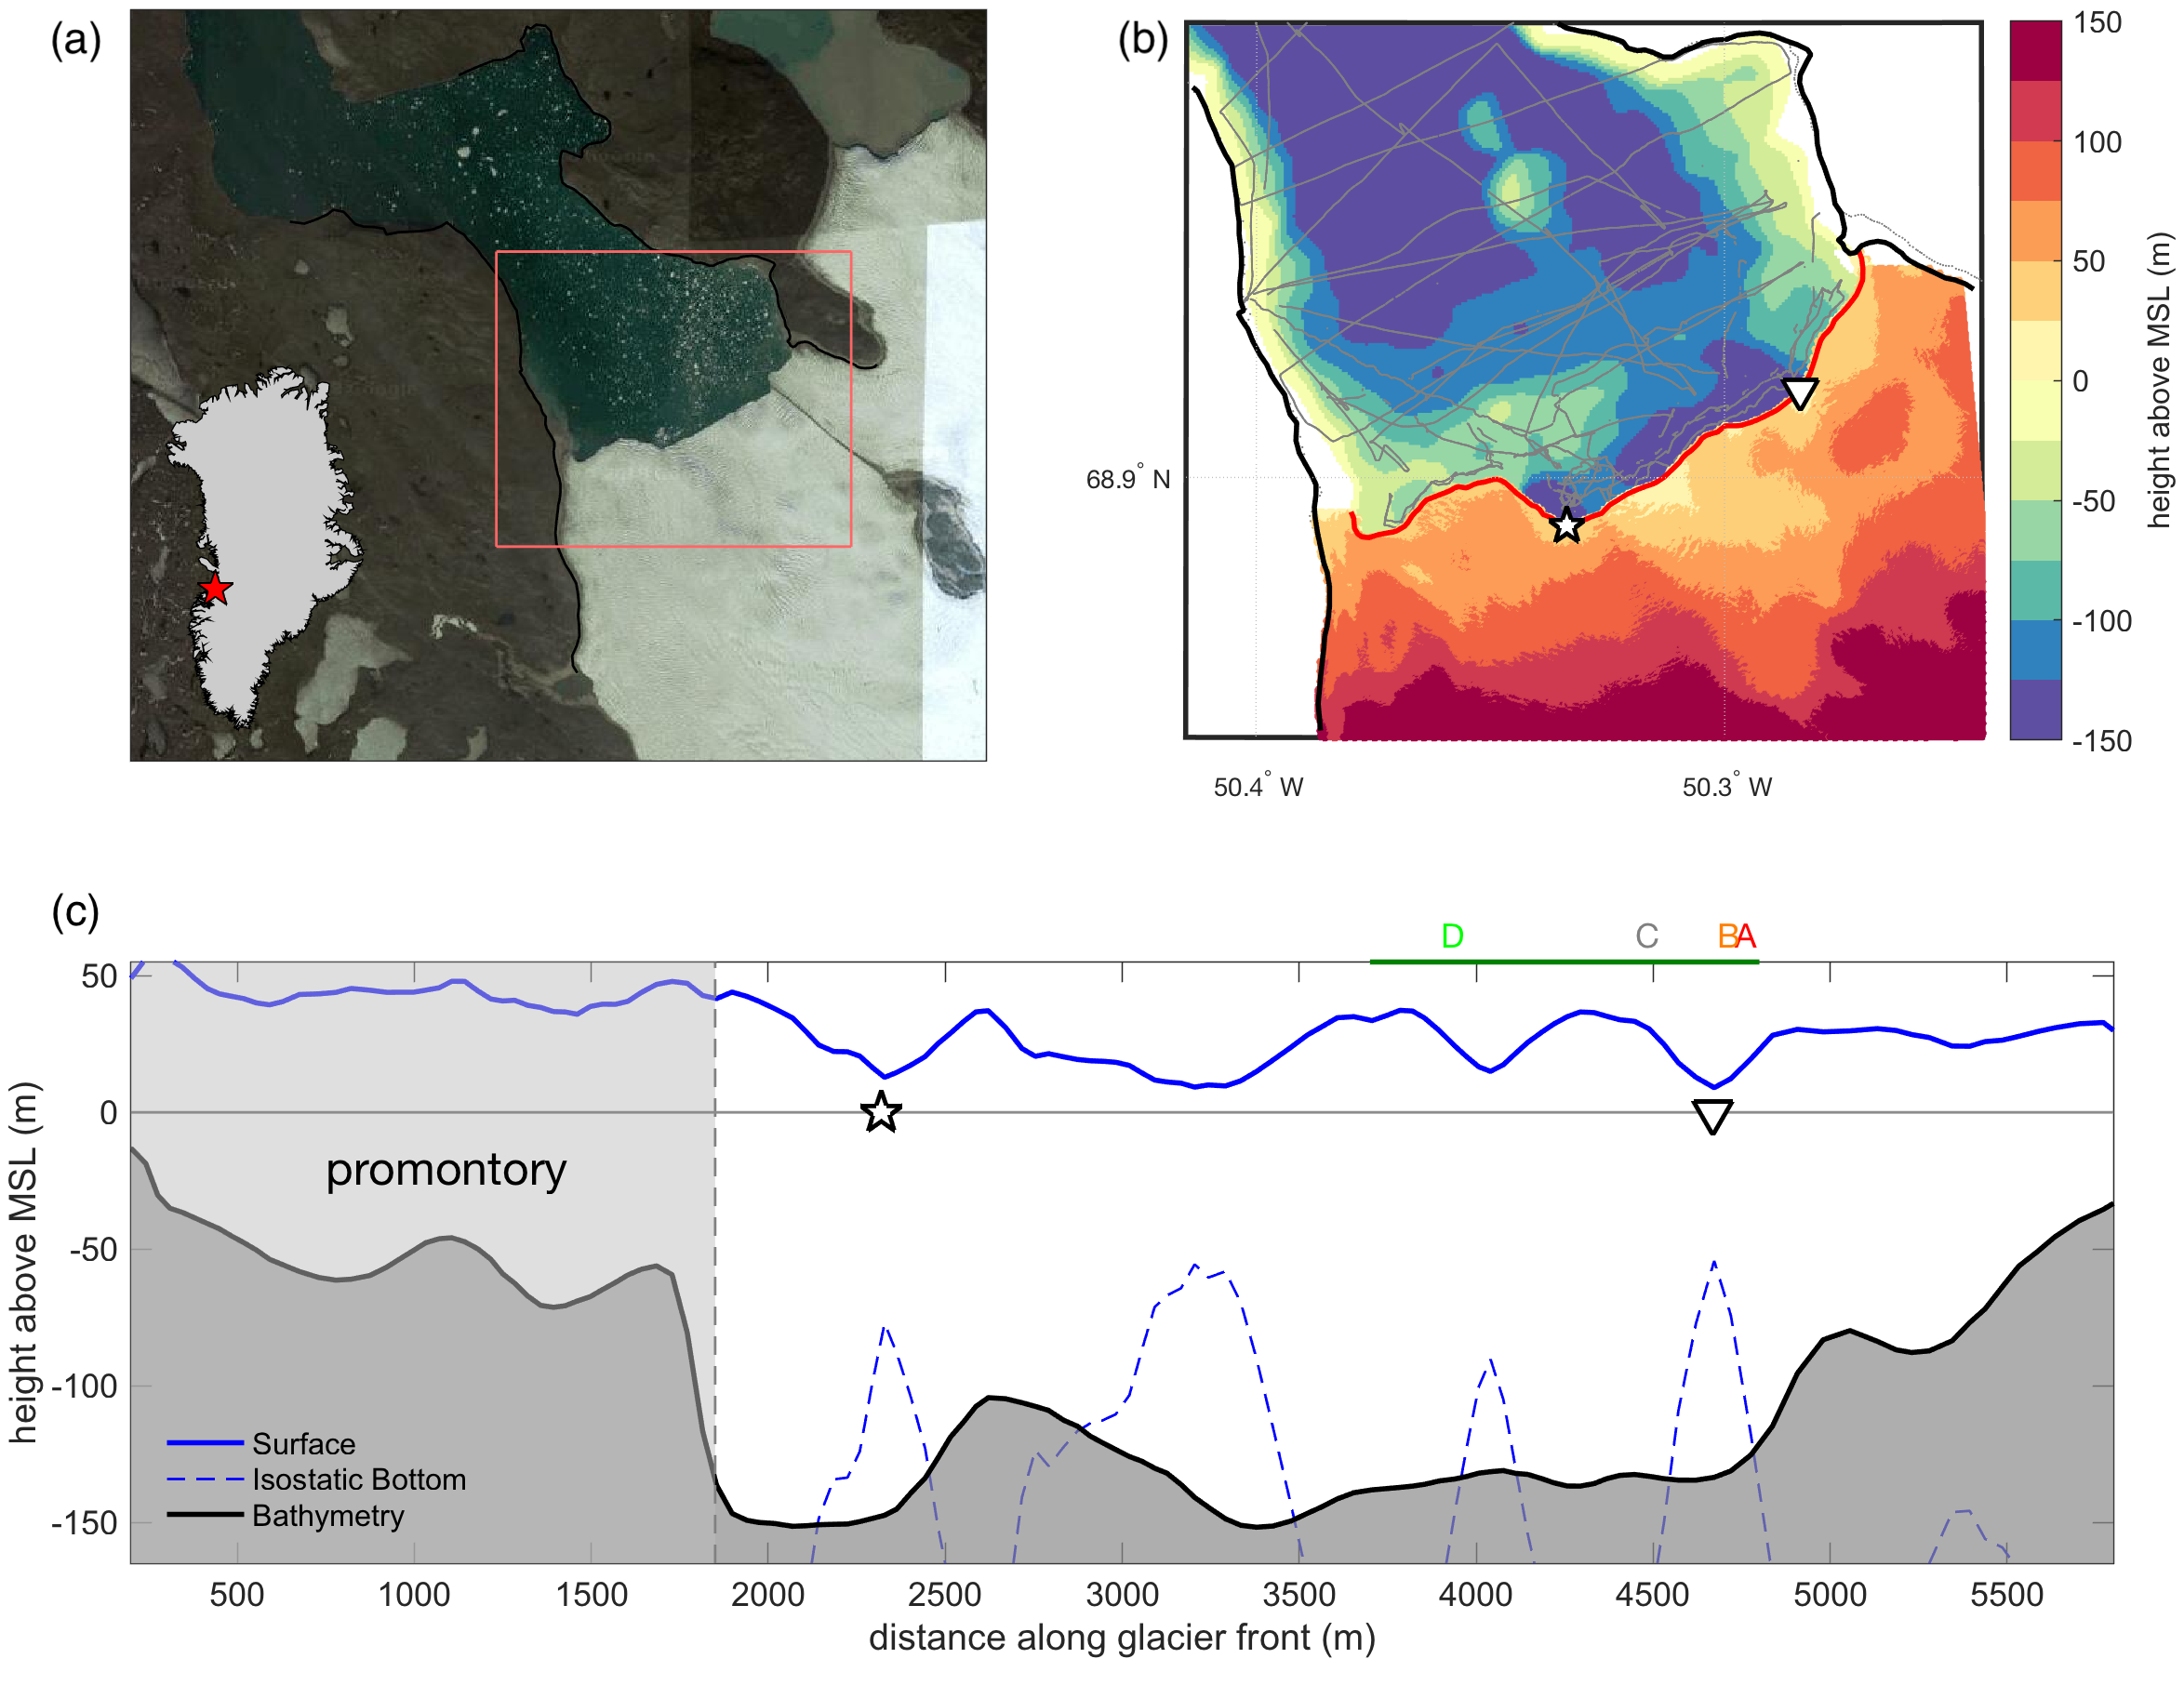
\includegraphics[width=\linewidth]{Figures/geometry4.png}
  \caption{(a) Map of the lower part of Sarqardliup Sermia, and Sarqardleq fjord. The inset of Greenland indicates the location of the glacier. (b) Gridded bathymetry from in-situ observations (readings indicated by gray dots). Also shown are the surface height from ArcticDEM, collected during an overflight on 22 March 2013; Digital Elevation Map created by the Polar Geospatial Center from DigitalGlobe, Inc. imagery. (c) Surface height (blue) and bathymetry (black) along glacier front. Also shown is the isostatic height of flotation, computed from the surface height and assuming a density 880 kg/m$^3$. Locations of two main plumes are highlighted in panels (b) and (c) by black symbols. The green horizontal line above panel (c) and the letters A-D indicate the locations of the front profiles shown in Fig \ref{fig:fronts}.}
  \label{fig:geometry}
  \end{center}
\end{figure*}

\subsection{Bathymetry} \label{bathy}

The existing bathymetry map of the fjord compiled from data collected during field work in 2012 and earlier \citep{Stevens:2016tx}, is supplemented with several additional near-terminus datasets from the 2013 field campaign. These consist of circa 39,000 depth readings taken with Jetyak and ship-mounted ADCPs. In addition, there are approximately 6000 readings from the boat-mounted NMEA bottom-range profiler and 6 readings from XCTDs deployed in the otherwise undersampled region of the main plume. Most of these readings are between 10--100 m from the glacier front. The revised bathymetry map (Fig \ref{fig:geometry}b) highlights a sill at depth $\sim$ 50 m that runs roughly parallel to the main glacier front at a distance of $\sim$1.5 km from the 2013 front position. This sill corresponds approximately to the location of the furthest advance of the glacier front in 1992. The sill furthermore separates the main basin of the fjord from a small, somewhat isolated, basin near the glacier front with slightly different water properties at depth (not shown). 

Fig \ref{fig:geometry}c shows the bathymetry at the glacier front in terms of $x$, the distance along the glacier front. The bathymetry can be split into two main regimes: For $x < 1800$ m (the promontory) the glacier is grounded in shallow waters and its surface heights are elevated substantially above floatation (see next section). From here on, we refer to the eastern part of the glacier ($x > 1800$ m) as the `main' glacier. In 2013, the front of the promontory was still coinciding with the above-mentioned sill, thus perched on bathymetry of  50 m depth or less. This part of the glacier front has also retreated since 2013 by several hundred meters (Fig S2). The main part of the glacier front is in waters of depth 130-150 m. A pronounced dip in bathymetry is found near the location of the main plume (distance $x = 2000 - 2400$ m along the front). A number of smaller dips are observed between $x = 3400 - 4700$ m. Beyond 4700 m the water depth decreases as one approaches the northeastern shoreline.

\subsection{Glacier surface topography} \label{surface}

An ArcticDEM overflight dated 22 March 2013 covers the full span of the Sarqardliup glacier front and some of the upstream region. This data provides digital elevation maps (DEMs), created by the Polar Geospatial Center from DigitalGlobe, Inc.~imagery. The data set has a horizontal resolution of 2 m and is capable of resolving individual crevasses on the glacier surface. As is also known from the field campaigns, the front of the glacier is heavily crevassed and furthermore features several pronounced dips in the surface elevation at the terminus. The ice cliff is highest (up to 50 m) and most uniform in the region of the promontory, while the main part of the glacier is much more variable with 4 distinct depressions that reach below 10 m surface elevation. A source of uncertainty is due the date of the ArcticDEM, which was collected 4 months prior to the main study period in July 2013. However, the above-water surface elevation is a relatively small contributor to the overall mass balance.

The coinciding high-resolution surface elevation and bathymetry data near the terminus enables us to compute the total ice thickness along the glacier front, $H(x)$, which allows for an estimation of the total ice flux (discussed below). 

Interestingly, the depressions in the surface elevation at the glacier front are all low enough to raise the isostatic bottom of the ice above the estimated depth of the local bathymetry. That is to say, if the glacier front was locally isostatic everywhere, the ice would be floating at the positions of the four dips shown in Fig \ref{fig:geometry}c. This assumes an average ice density of 883 kg m$^{-3}$ (obtained as a mean of the lowest and highest commonly used glacier and ice shelf densities, 850 and 917 kg m$^{-3}$). The ice would be grounded everywhere else. In particular, it is elevated substantially beyond its isostatic height in the region of the promontory. The locally-isostatic bottom of the ice is indicated in Fig \ref{fig:geometry}c (blue dashed line). It should be noted that the surrounding ice and the associated stiffness of the glacier will likely prevent the ice from assuming local isostasy everywhere along the glacier front. However, the isostatic bottom can be used to compute a lower bound on the ice thickness in regions where the ice may be floating. It may be speculated that the ice is floating in these regions due to undercutting by submarine melt (which in turn is associated with rising discharge plumes, as discussed in Section \ref{melting}). 

\section{Ice flux and retreat}

\subsection{Ice velocity and advective ice flux} \label{vels}

Several ice-velocity data fields of the lower part of the glacier are available for the years 2009 -- 2015 from InSAR data \citep{Joughin:uFAgCs4K}. The mean flow velocity at the glacier front (averaged over all available fields) is $\sim 350$ m yr$^{-1}$ with minima at the edges of the glacier. There is a notable peak in ice velocity (up to 700 m yr$^{-1}$) near the location of the main plume (Fig \ref{fig:vels}). A second stream of elevated velocities is found near $x = 4000$ m and is more pronounced somewhat further upstream. The drainage location of this second stream coincides with that of the second discharge plume. It is worth noting that the spatial distribution of velocities was remarkably consistent during summer months from 2012--2014 (Fig  \ref{fig:vels}b), followed by a substantial slow-down in 2015 (not shown). In what follows, we will consider the 2012--2014 summer (May--September) mean velocity profile along the glacier front. Using the mean July velocities instead does not change the results notably. 

%It is worth noting that the retreat of the main part of the glacier is more pronounced than that of the promontory. Aside from these differences, the rate of retreat is spatially close to uniform along the glacier front ($80 \pm 4$ m yr$^{-1}$ between 2004 and 2016).4
